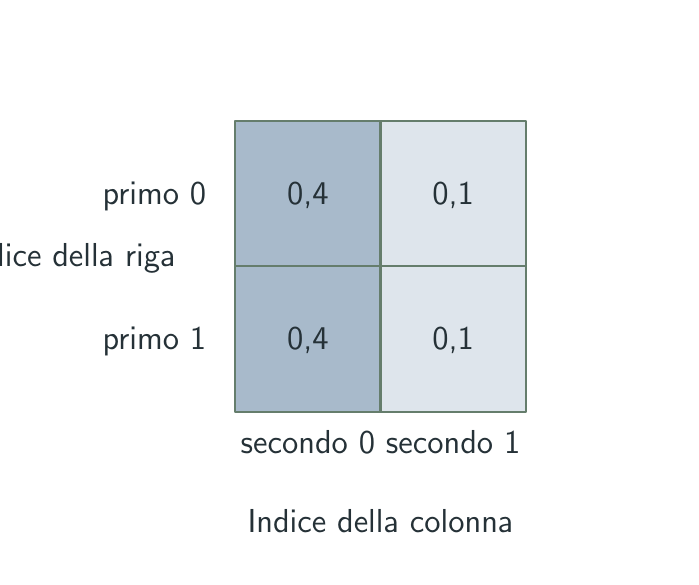
\begin{tikzpicture}[x=.75pt,y=-.75pt,line join=round,line cap=round]
\path[use as bounding box] (0,0) rectangle (310,255);
\path[draw={rgb,255:red,101;green,125;blue,108},fill={rgb,255:red,74;green,111;blue,147},line width=0.75pt,fill opacity=0.48000000000000004] (100,45) rectangle (170,115);
\node[inner sep=0pt,outer sep=0pt,anchor=base,font={\sffamily\fontsize{12}{14.4}\selectfont},text={rgb,255:red,37;green,49;blue,55}] at (135,85) {0,4};
\path[draw={rgb,255:red,101;green,125;blue,108},fill={rgb,255:red,74;green,111;blue,147},line width=0.75pt,fill opacity=0.18] (170,45) rectangle (240,115);
\node[inner sep=0pt,outer sep=0pt,anchor=base,font={\sffamily\fontsize{12}{14.4}\selectfont},text={rgb,255:red,37;green,49;blue,55}] at (205,85) {0,1};
\path[draw={rgb,255:red,101;green,125;blue,108},fill={rgb,255:red,74;green,111;blue,147},line width=0.75pt,fill opacity=0.48000000000000004] (100,115) rectangle (170,185);
\node[inner sep=0pt,outer sep=0pt,anchor=base,font={\sffamily\fontsize{12}{14.4}\selectfont},text={rgb,255:red,37;green,49;blue,55}] at (135,155) {0,4};
\path[draw={rgb,255:red,101;green,125;blue,108},fill={rgb,255:red,74;green,111;blue,147},line width=0.75pt,fill opacity=0.18] (170,115) rectangle (240,185);
\node[inner sep=0pt,outer sep=0pt,anchor=base,font={\sffamily\fontsize{12}{14.4}\selectfont},text={rgb,255:red,37;green,49;blue,55}] at (205,155) {0,1};
\node[inner sep=0pt,outer sep=0pt,anchor=base,font={\sffamily\fontsize{12}{14.4}\selectfont},text={rgb,255:red,37;green,49;blue,55}] at (135,205) {secondo 0};
\node[inner sep=0pt,outer sep=0pt,anchor=base,font={\sffamily\fontsize{12}{14.4}\selectfont},text={rgb,255:red,37;green,49;blue,55}] at (205,205) {secondo 1};
\node[inner sep=0pt,outer sep=0pt,anchor=base east,font={\sffamily\fontsize{12}{14.4}\selectfont},text={rgb,255:red,37;green,49;blue,55}] at (86,85) {primo 0};
\node[inner sep=0pt,outer sep=0pt,anchor=base east,font={\sffamily\fontsize{12}{14.4}\selectfont},text={rgb,255:red,37;green,49;blue,55}] at (86,155) {primo 1};
\node[inner sep=0pt,outer sep=0pt,anchor=base,font={\sffamily\fontsize{12}{14.4}\selectfont},text={rgb,255:red,37;green,49;blue,55}] at (170,243) {Indice della colonna};
\begin{scope}[shift={(20,115)},rotate=90]
\node[inner sep=0pt,outer sep=0pt,anchor=base,font={\sffamily\fontsize{12}{14.4}\selectfont},text={rgb,255:red,37;green,49;blue,55}] at (0,0) {Indice della riga};
\end{scope}
\end{tikzpicture}
